\input{../preamble.tex}

\lecturenumber{10}
\title{Memory}
\version{2.0.0}

\begin{document}

\begin{frame}[plain, noframenumbering]
    \titlepage
\end{frame}

\begin{slide}

	\slidetitle{The Memory Wall Problem}
	
	\begin{minipage}{0.45\textwidth}
	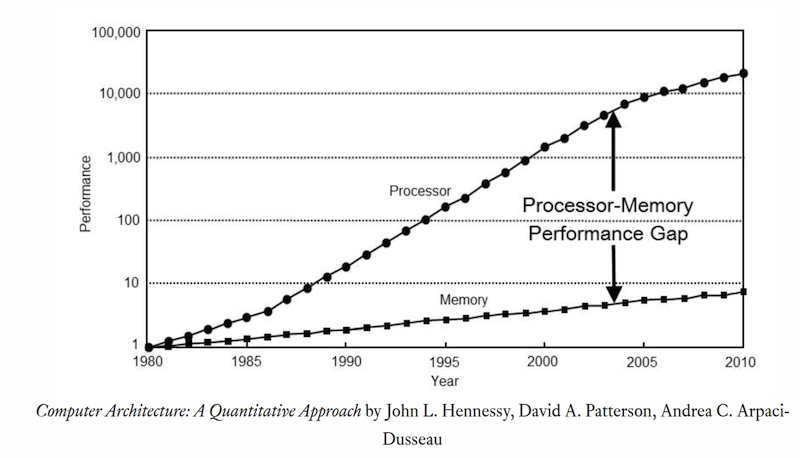
\includegraphics[width=60mm]{memory-wall.png}
	\end{minipage}
	\hfill
	\begin{minipage}{0.45\textwidth}
	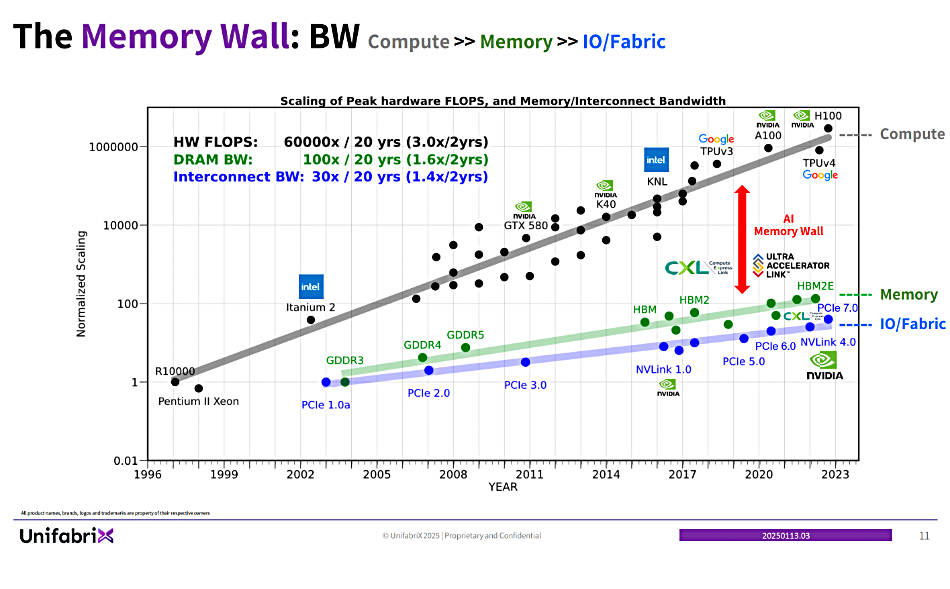
\includegraphics[width=60mm]{memory-wall-2.jpg}
	\end{minipage}
	
\vspace{2mm}

Memory is one of the most important topics in OS.
\bigskip

Hardware and software development are both very active (commercially and academically).

\end{slide}

\begin{slide}

    \slidetitle{The early operating system}

    \begin{minipage}{0.3\textwidth}
        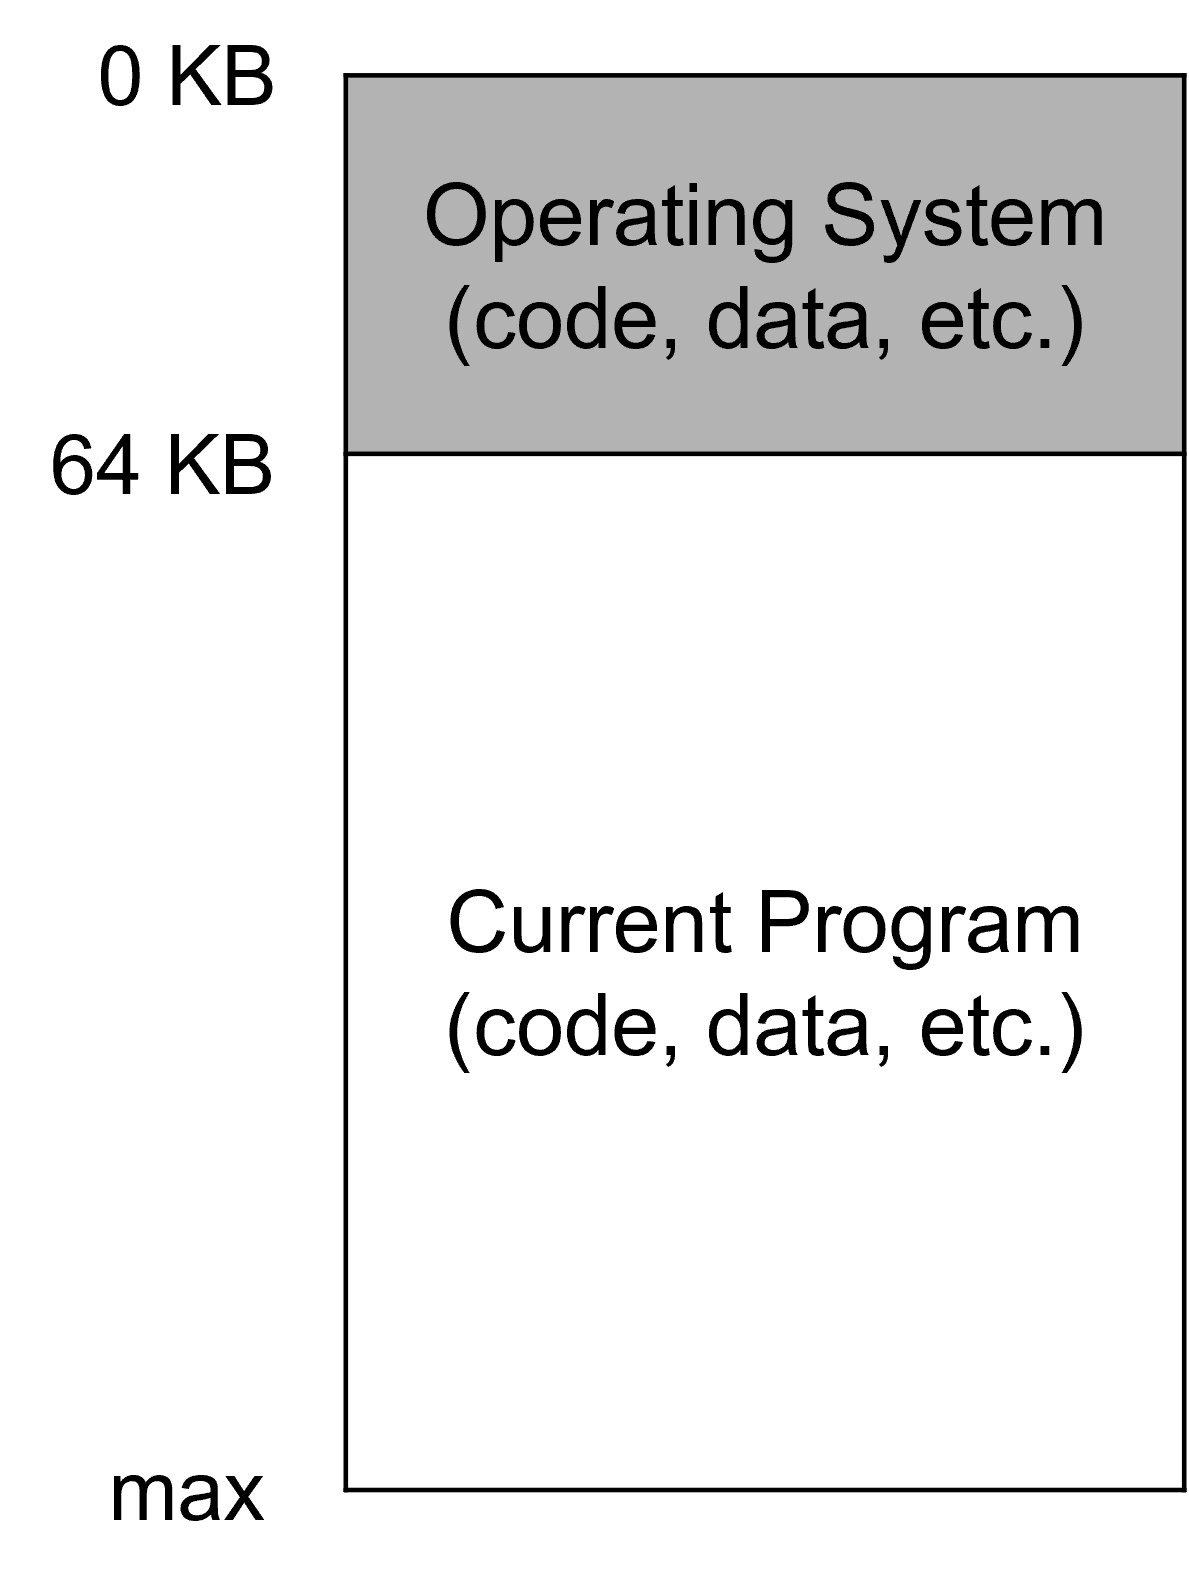
\includegraphics[width=40mm]{early-os-mem.png}
    \end{minipage}
    \hfill
    \begin{minipage}{0.65\textwidth}
        (Almost) No hardware abstraction.
        \bigskip

        OS is a set of routines (libraries).
        \bigskip

        A single running program in physical memory.
    \end{minipage}

\end{slide}

\begin{slide}

    \slidetitle{Multiple people start sharing a computer}

    Timeshare: One user runs for a bit, saves everything to disk, then load another.
    \bigskip

    But it is very slow.

\end{slide}

\begin{slide}

    \slidetitle{Writing from disk to memory is slow...but registers are fast}

    \begin{minipage}{0.3\textwidth}
    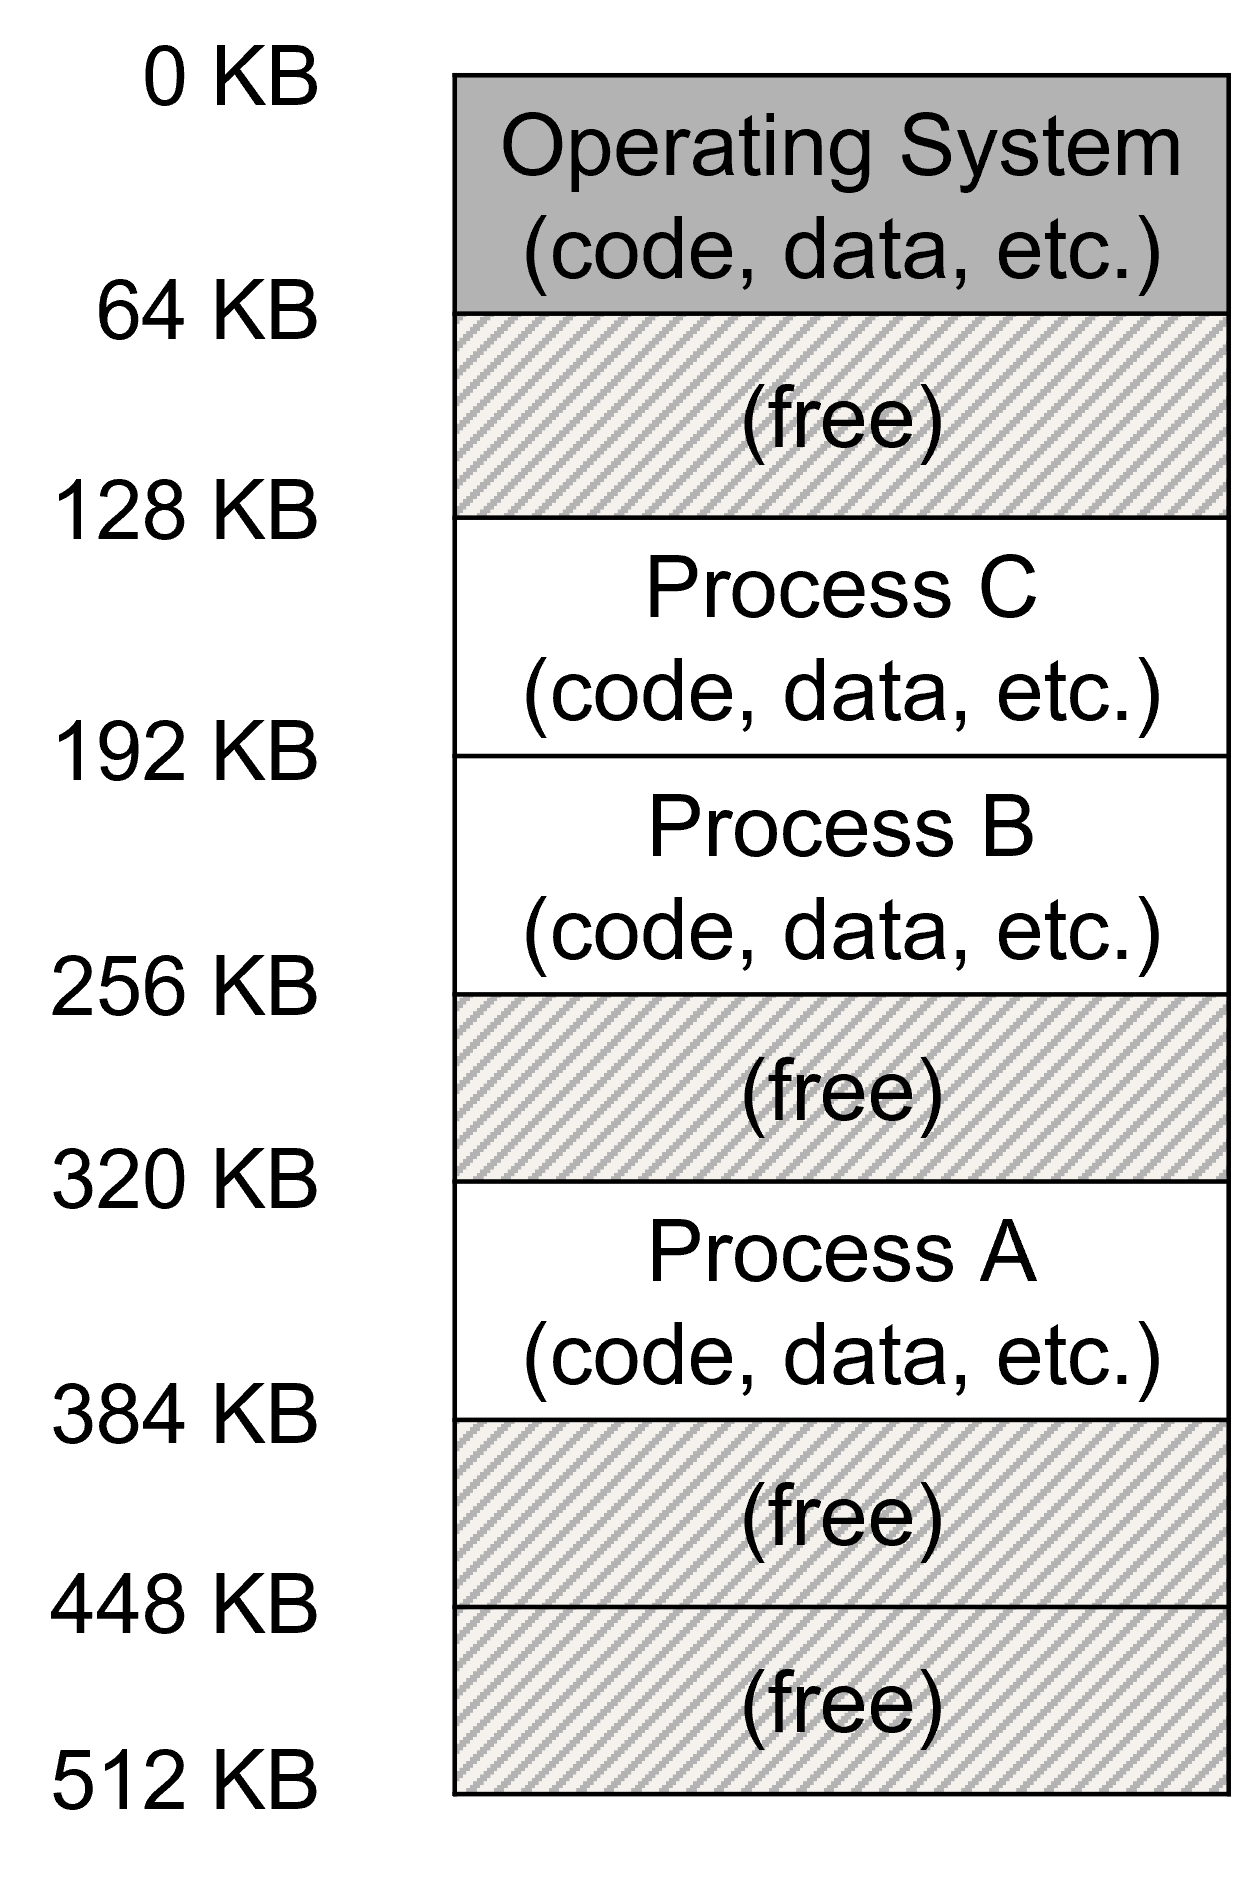
\includegraphics[width=40mm]{multi-process-mem.png}
    \end{minipage}
    \hfill
    \begin{minipage}{0.65\textwidth}
        A second try - leaves everything in memory, but switch between them.
        \bigskip

        Each process gets 64 KB space from physical memory.
        \bigskip

        But there is no abstraction - any problems?
    \end{minipage}

\end{slide}

\begin{slide}

    \slidetitle{Create an abstraction – address space}

	
    \begin{minipage}{0.3\textwidth}
        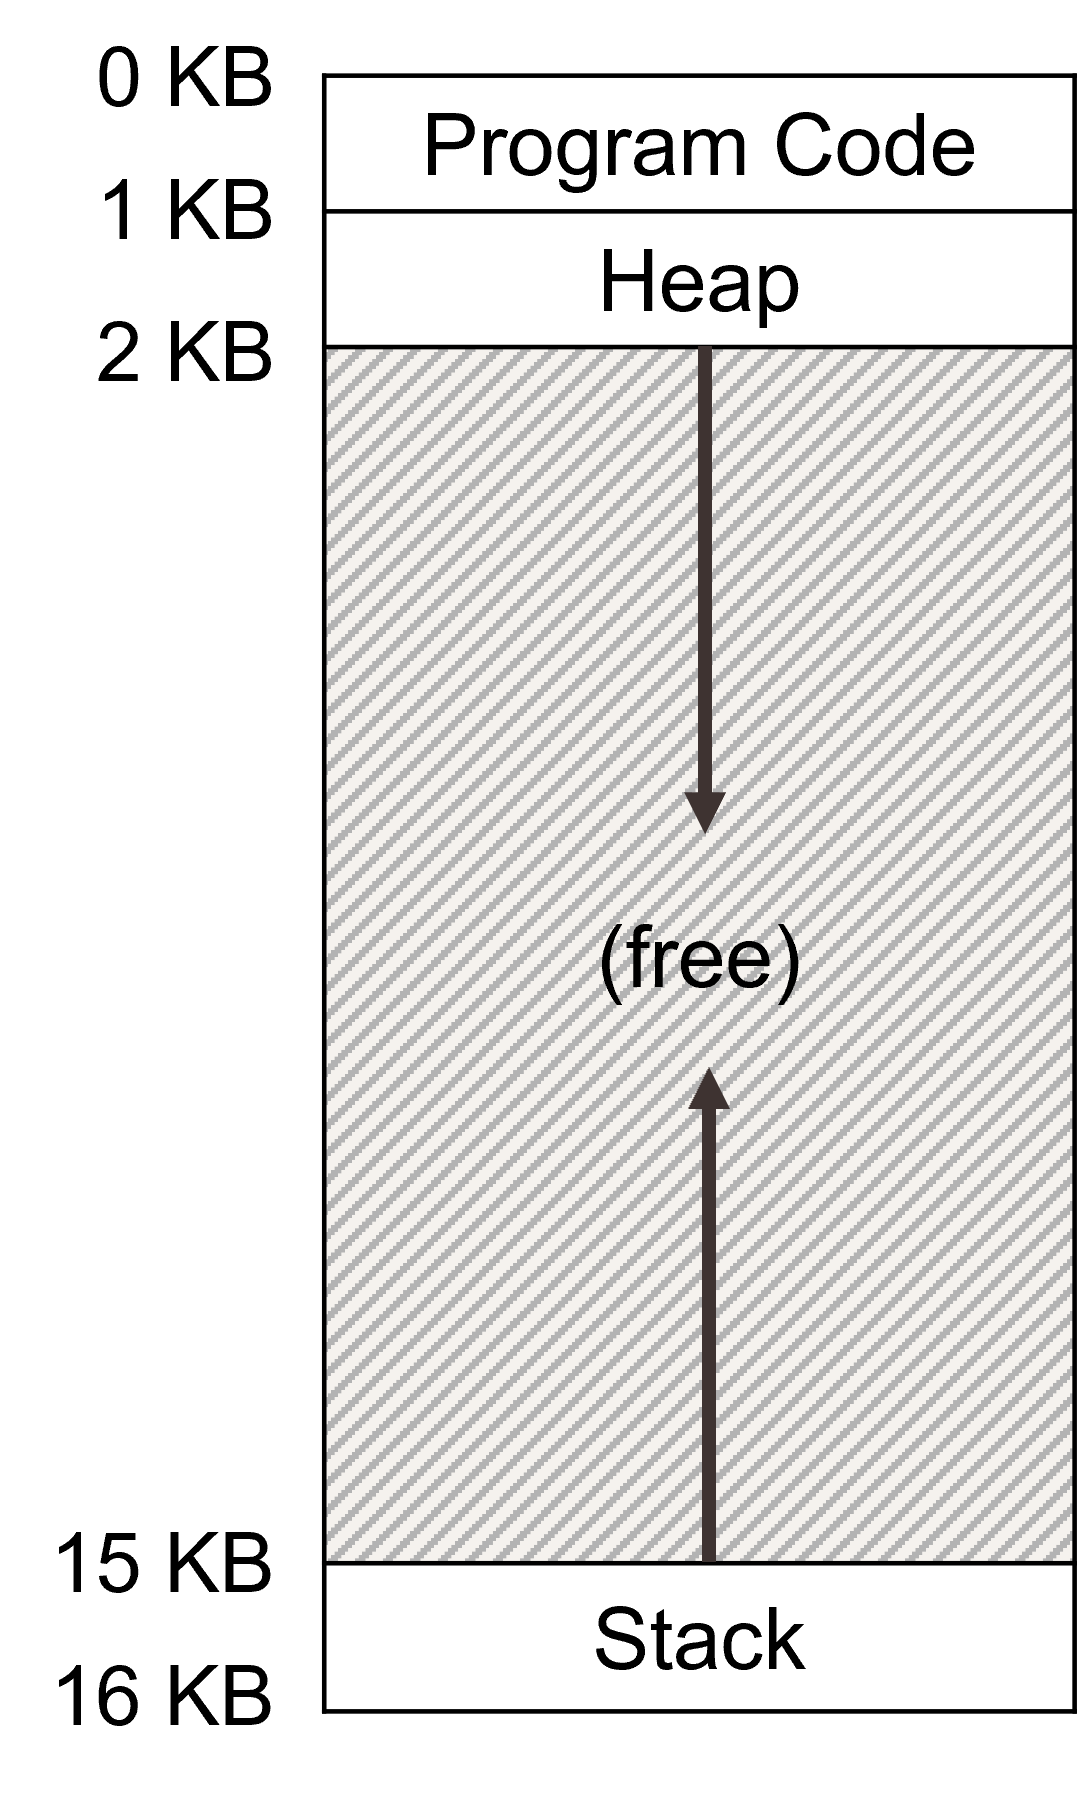
\includegraphics[width=40mm]{address-space-segments.png}
    \end{minipage}
    \hfill
    \begin{minipage}{0.65\textwidth}
        An address space is the running program's view of memory in the system.
        \bigskip

        Code: where instructions live
        \bigskip

        Heap: dynamic data (malloc'd data)
        \bigskip

        Stack: local variables, arguments to routines, return values, etc.
    \end{minipage}
    
\end{slide}

\begin{slide}

    \slidetitle{Create an abstraction – address space}
    
    \inputminted{c}{memory-exp.c}
    \bigskip

    Virtual address or physical memory?
    
\end{slide}

\begin{slide}

    \slidetitle{Create an abstraction – address space}

	\vspace{-5mm}
	
    Difference?
    \medskip

    \begin{minipage}{0.3\textwidth}
        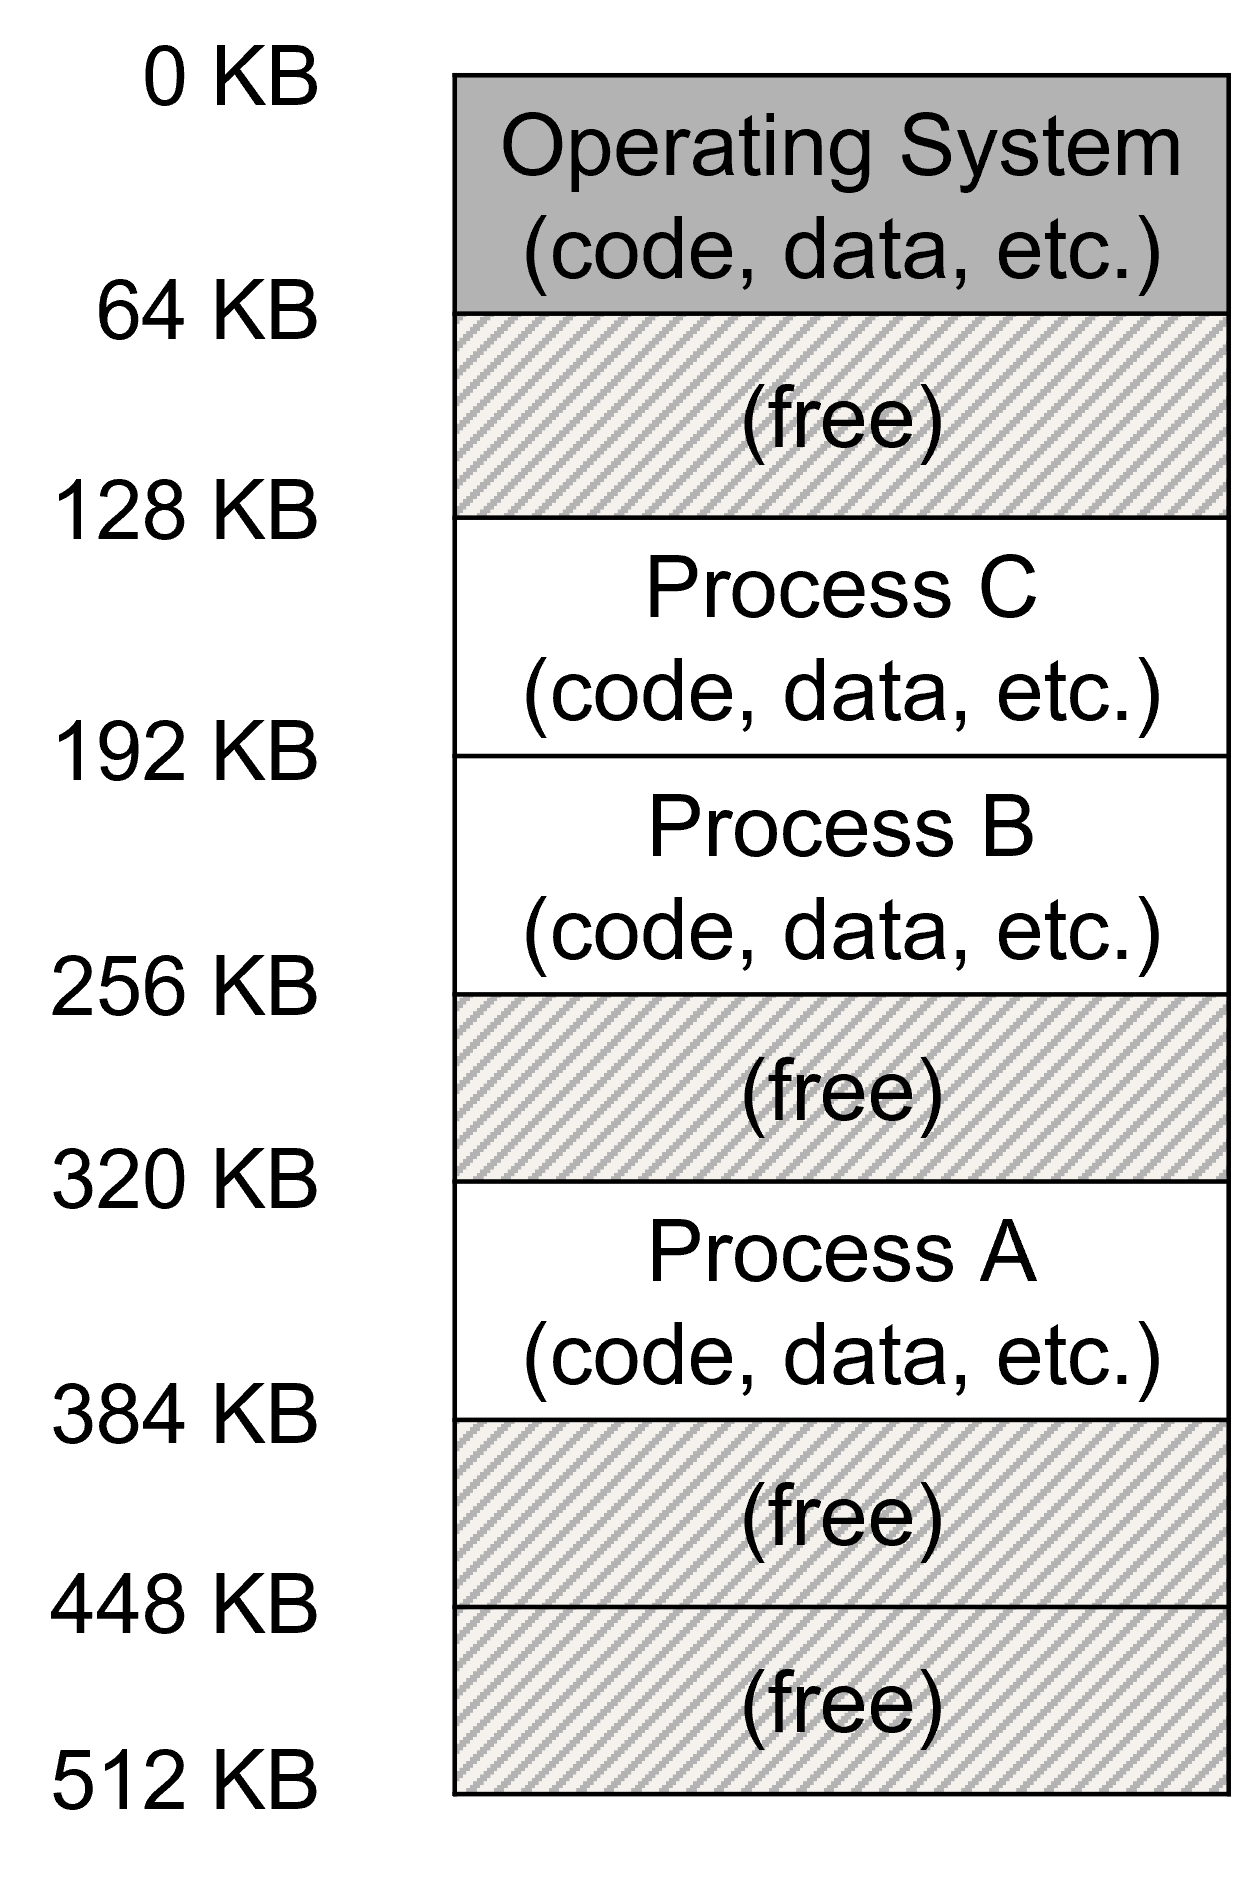
\includegraphics[width=30mm]{multi-process-mem.png}
    \end{minipage}
    \hspace{10mm}
    \begin{minipage}{0.3\textwidth}
        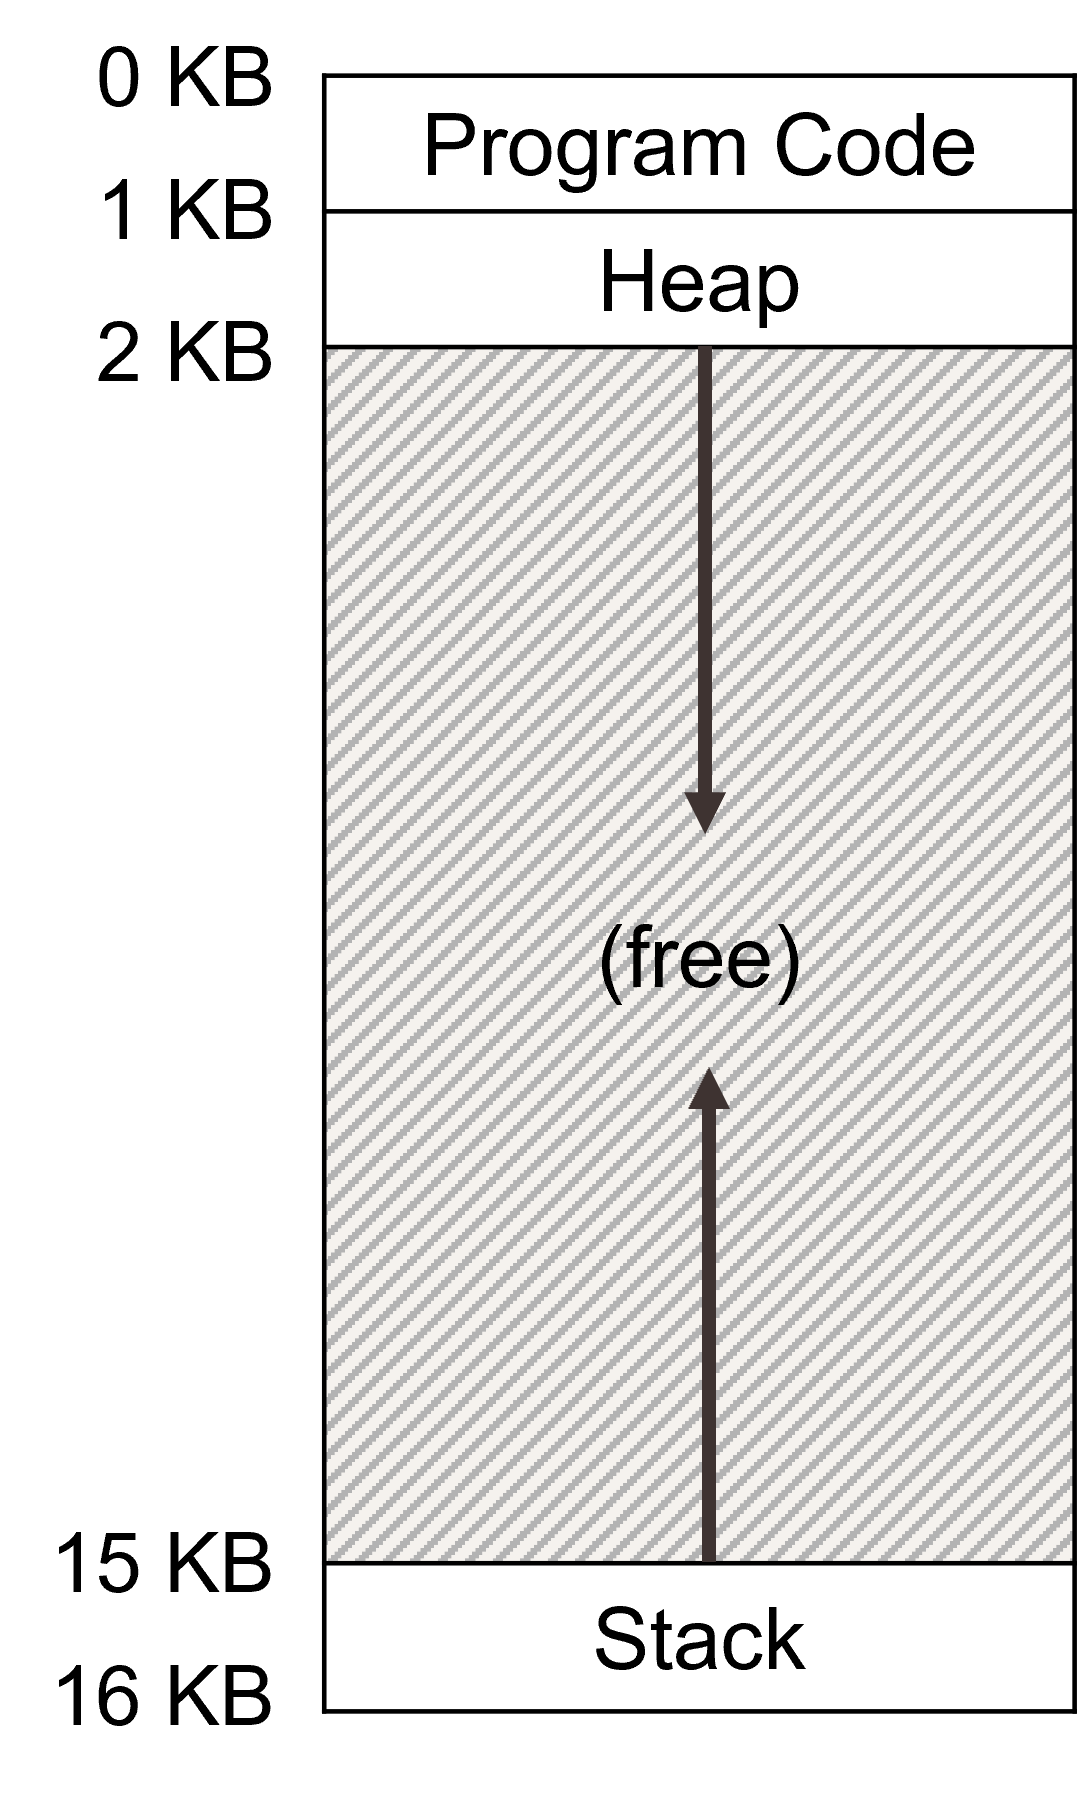
\includegraphics[width=30mm]{address-space-segments.png}
    \end{minipage}
    \medskip

    How can the OS build this abstraction of a private, potentially large address space for multiple running processes (all sharing memory) on top of a single, physical memory?

\end{slide}

\begin{slide}

	\slidetitle{The memory management unit (MMU)}
	
	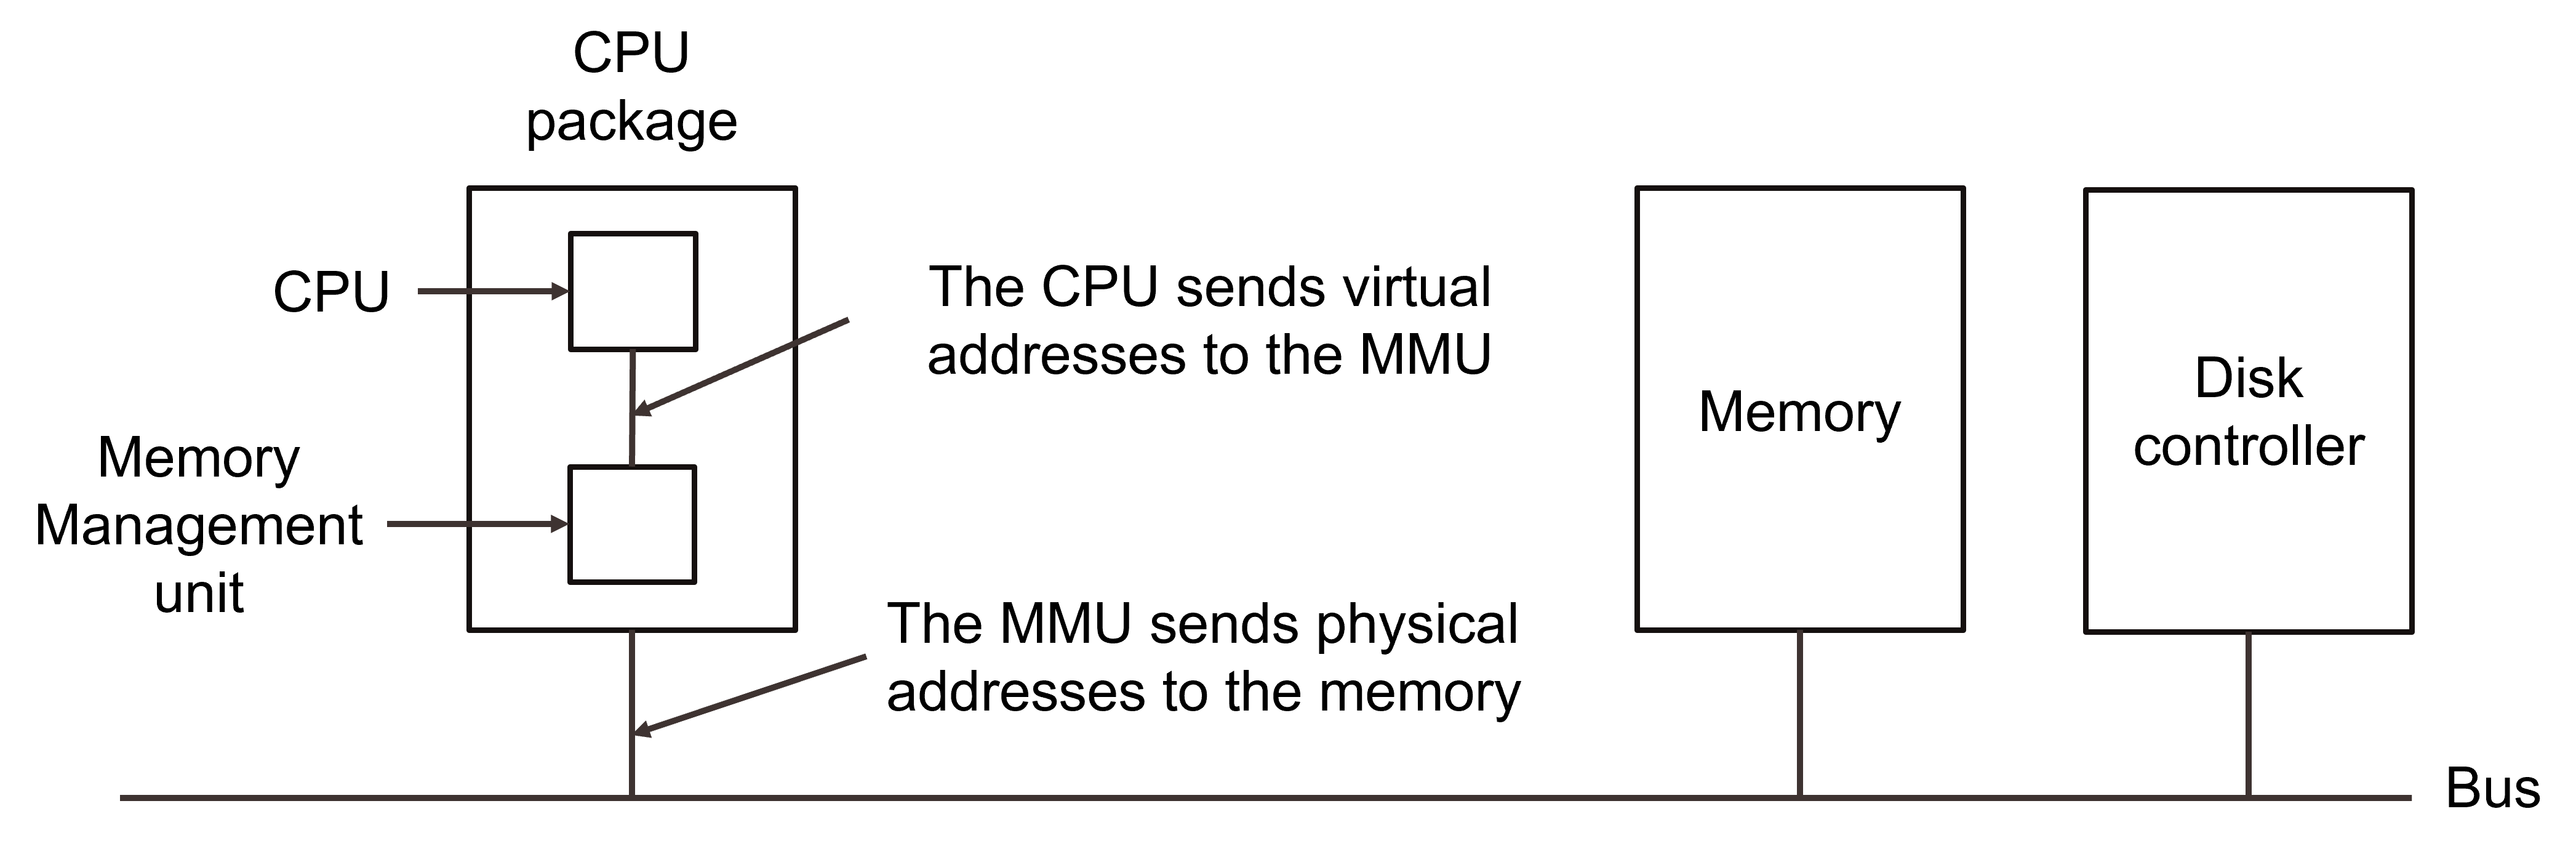
\includegraphics[width=100mm]{mmu.png}

\end{slide}

\begin{comment}
\begin{slide}
    
    \slidetitle{How Should We Implement Virtual Mapping?}

    What are your ideas for mapping a process's virtual memory to physical
    memory?

\end{slide}
\end{comment}

\begin{slide}

    \slidetitle{Virtual Memory Checklist}

    \begin{itemize}
      \item Multiple processes must be able to co-exist
      \item Processes are not aware they are sharing physical memory
      \item Processes cannot access each others data (unless allowed explicitly)
      \item Performance close to using physical memory
      \item Limit the amount of fragmentation (wasted memory)
    \end{itemize}

\end{slide}
  
\begin{slide}

    \slidetitle{Base and limit registers}

    \begin{minipage}{0.4\textwidth}
        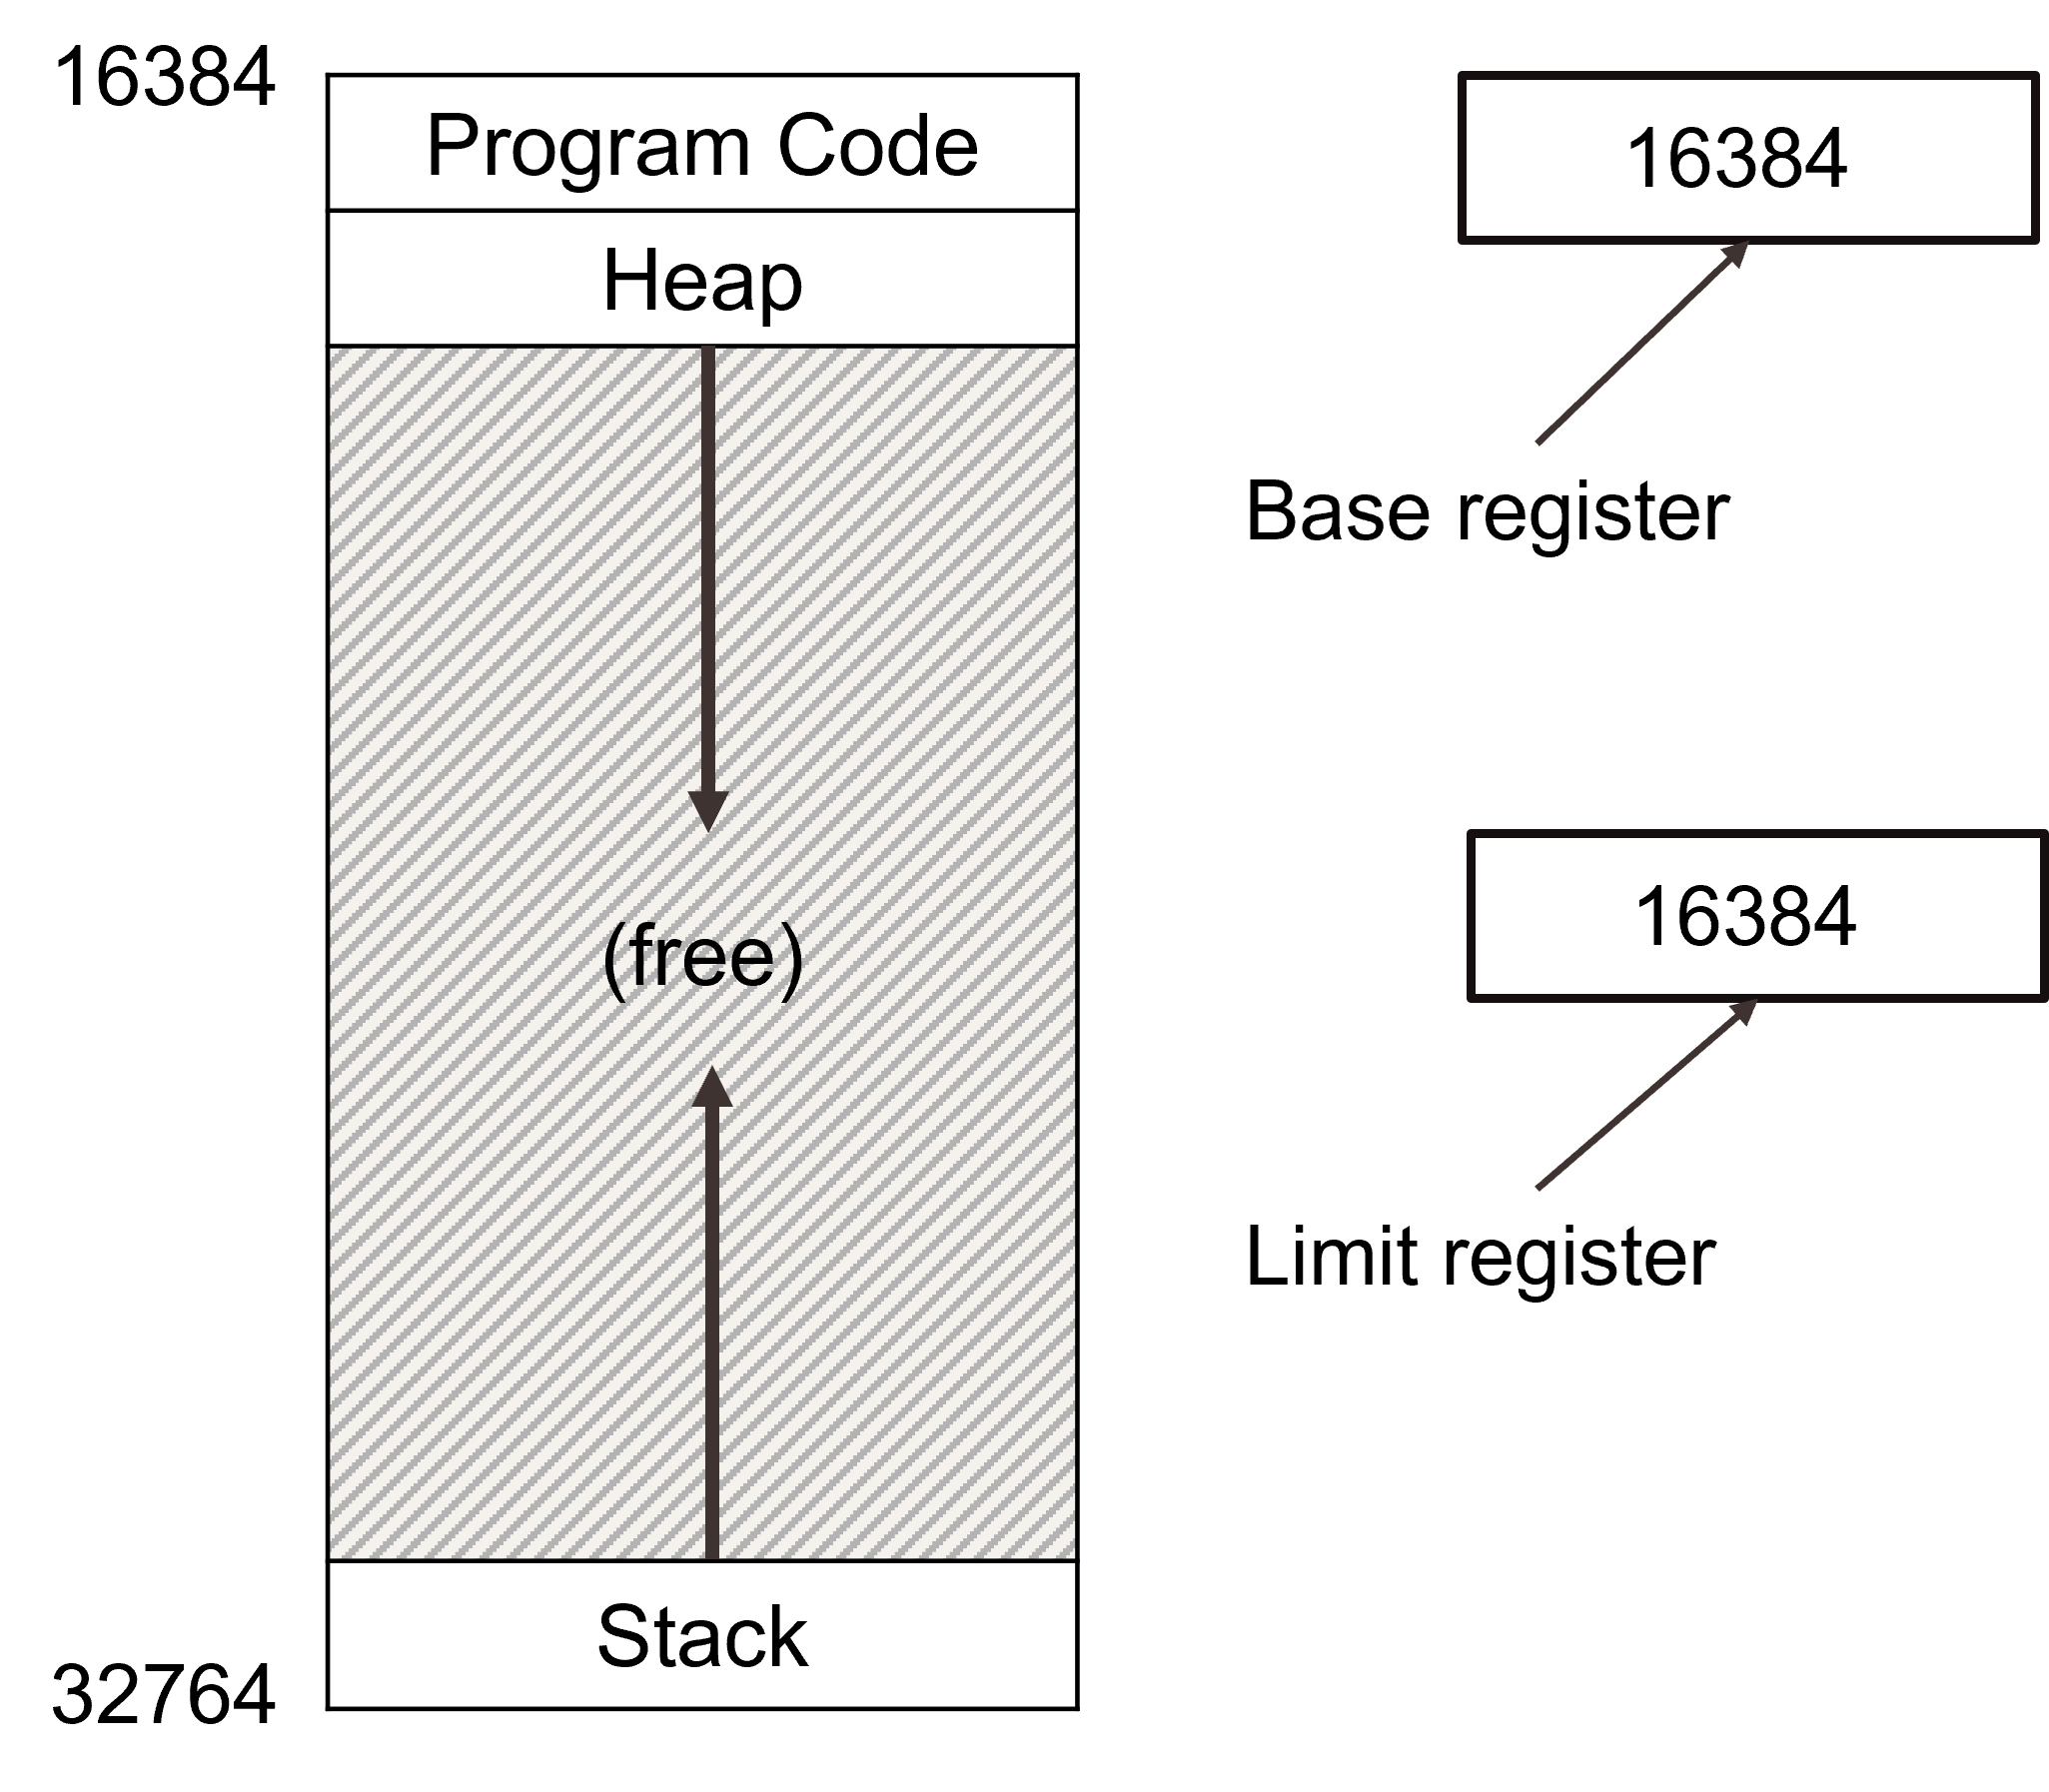
\includegraphics[width=50mm]{base-limit-reg.png}
    \end{minipage}
    \hfill
    \begin{minipage}{0.58\textwidth}
        The simple solution: Each CPU has two special hardware registers: base and limit.
        \bigskip

        When a process is run, the addresses are loaded to these registers.
        \bigskip

        An addition and a comparion on every memory reference.
        \bigskip
    \end{minipage}

\end{slide}

\begin{slide}

    \slidetitle{Remember That Memory is Byte Addressable}

    The smallest unit you can use to address memory is one byte
    \medskip

    You can read or write one byte at a time at minimum
    \medskip

    Each ``address'' is like an index of an array

\end{slide}

\begin{slide}

    \slidetitle{Segmentation or Segments are Coarse Grained}

    Divide the virtual address space into segments for: code, data, stack, and heap


    Each segment is a variable size, and can be dynamically resized

    \leftspace{}This is an old legacy technique that's no longer used
    \medskip

    Segments can be large and very costly to relocate

    \leftspace{}It also leads to fragmentation (gaps of unused memory)
    \medskip

    No longer used in modern operating systems

\end{slide}

\begin{slide}
    
    \slidetitle{First Insight: Divide Memory into Fixed-Sized Chunks}

    \centering
    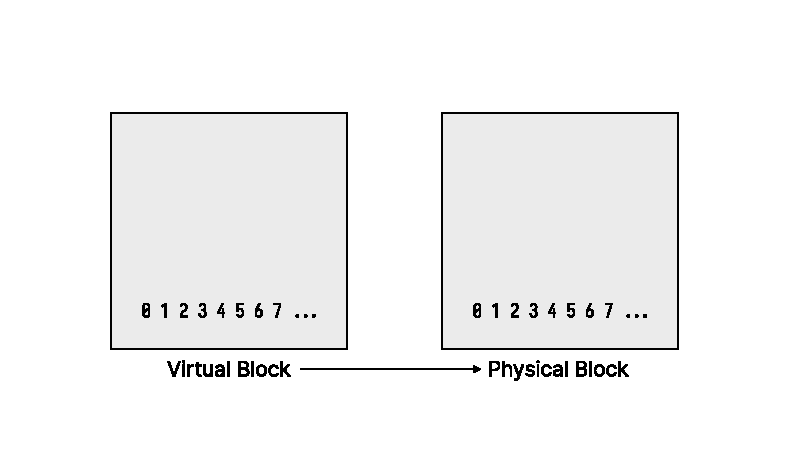
\includegraphics{virt-to-phy-block.eps}

\end{slide}
  
\begin{slide}

    \slidetitle{Paging}

    One technique is to divide memory up into fixed-size pages (typically 4096 bytes or 4 KB)
	\begin{itemize}
		\item A page in virtual memory is called a page
		\item A page in physical memory is called a frame
	\end{itemize}
	
\end{slide}

\begin{comment}
\begin{slide}

	\slidetitle{A Library Analoge}
	
	Imagine you are in a rare book library 
	
	\leftspace{} - You can’t browse the shelves yourself 
	
	\leftspace{} - You can only read books in the reading room.
	
	\bigskip
	
	You have to make a request for the records to be transferred to the reading room.
	
	\leftspace{} - You have to request at least a page at a time.
	
	\bigskip
	
	The librarian puts the request through, the system fetches it from the back room.
	
	\bigskip
	
	Once the book is in the reading room, you can read a word (byte) at a time.
	
\end{slide}

\end{comment}

\begin{slide}

    \slidetitle{You Typically Do Not Use All 64 Virtual Address Bits}

    CPUs may have different levels of virtual addresses you can use

    \leftspace{}Implementation ideas are the same
    \medskip

    We'll assume a 39 bit virtual address space used by RISC-V and other
    architectures

    \leftspace{}Allows for 512 GiB of addressable memory (called Sv39)
    \medskip

    Implemented with a page table indexed by Virtual Page Number (VPN)

    \leftspace{}Looks up the Physical Page Number (PPN)

\end{slide}

\begin{slide}

    \slidetitle{The Page Table Translates Virtual to Physical Addresses}
	\vspace{-5mm}
	
    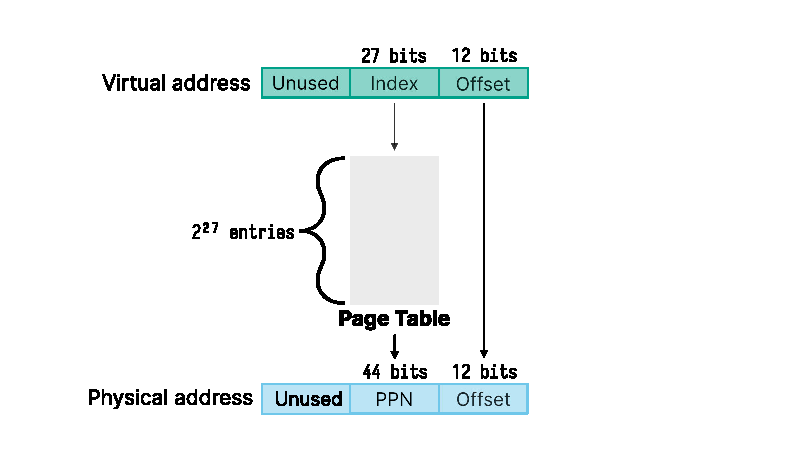
\includegraphics[width=120mm]{single-level-page-table.eps}
	\vspace{-3mm}
	
\end{slide}



\begin{slide}

    \slidetitle{The Page Table Entry (PTE) Also Stores Flags in the Lower Bits}
	\vspace{-16mm}
	
    \begin{center}
      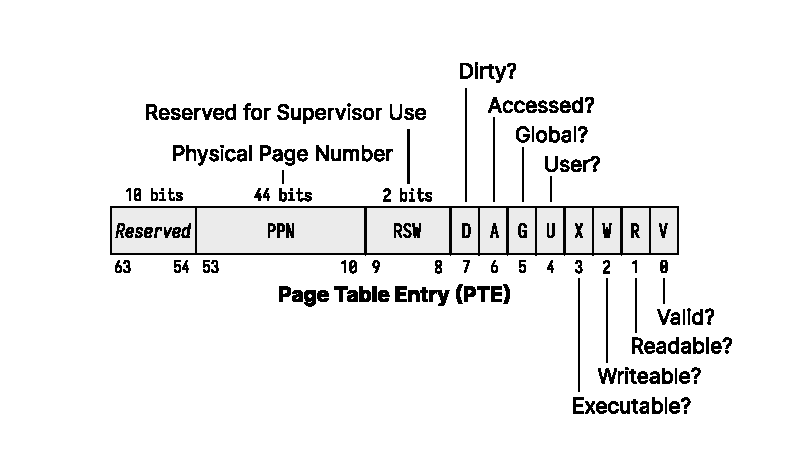
\includegraphics{pte.eps}
	  \vspace{-10mm}
    \end{center}

\end{slide} 

\begin{slide}

    \slidetitle{The Kernel Handles Translating Virtual Addresses}

    Considering the following page table:
    \begin{center}
    {\ttfamily
    \begin{tabular}{ll}
      VPN  & PPN  \\
      0x0 & 0x1 \\
      0x1 & 0x4 \\
      0x2 & 0x3 \\
      0x3 & 0x7 \\
    \end{tabular}}
    \end{center}
    \medskip

    We would get the following virtual $\rightarrow$ physical address translations:
    \begin{center}
    \texttt{0x0AB0} $\rightarrow$ 

    \texttt{0x1FA0} $\rightarrow$ 

    \texttt{0x2884} $\rightarrow$ 

    \texttt{0x32D0} $\rightarrow$ 
    \end{center}

\end{slide}

\begin{slide}

    \slidetitle{Page Translation Example Problem}

    Assume you have a 8-bit virtual address, 10-bit physical address

    \leftspace{}and each page is 64 bytes
    \medskip

    \begin{itemize}
      \item How many virtual pages are there? \onslide<2->{$\mathsf{\frac{2^8}{2^6} = 4}$}
      \item How many physical pages are there? \onslide<2->{$\mathsf{\frac{2^{10}}{2^6} = 16}$}
      \item How many entries are in the page table? \onslide<2->{$\mathsf{4}$}
      \item Given the page table is \texttt{{[0x2, 0x5, 0x1, 0x8]}}

            \hspace{2em} what's the physical address of \texttt{0xF1}?

            \onslide<2->{\texttt{0x231}}
    \end{itemize}

\end{slide}


\begin{slide}

    \slidetitle{Each Process Gets Its Own Page Table}

    When you \texttt{fork} a process, it will copy the page table from the parent

    \leftspace{}Turn off the write permission so the kernel can implement
    copy-on-write
    \medskip

    The problem is there are $\mathsf{2^{27}}$ entries in the page table, each
    one is 8 bytes

    \leftspace{}This means the page table would be 
    \medskip

    Note that RISC-V translates a 39-bit virtual to a 56-bit physical address

    \leftspace{}It has 10 bits to spare in the PTE and could expand

    \leftspace{}Page size is 4096 bytes (size of offset field)

\end{slide}

\begin{slide}

    \slidetitle{We Use Pages for Memory Translation}

    Divide memory into blocks, so we only have to translate once per block
    \medskip

    Use page tables (array of PTEs) to access the PPN (and flags)
    \medskip

    New problem: these page tables are always huge!

\end{slide}

\end{document}
